\begin{center}\small
\begin{tikzpicture}[x=1.25cm,y=6.5cm]
  \def\cval{0.666666} % c = 2/3
  \fill[blue!60!gray, opacity=0.28]
    (0,0) -- (1,\cval) -- (3,0) -- cycle;
  \draw[thick, blue!75!black] (0,0) -- (1,\cval) -- (3,0) -- (0,0);
  \draw[->] (-0.3,0) -- (3.35,0) node[right, font=\small] {$x$};
  \draw[->] (0,-0.05) -- (0,0.78) node[above, font=\small] {$f(x)$};

  \foreach \xb/\lbl in {0/$0$,1/$1$,3/$3$}{
    \draw (\xb,0) -- ++(0,-0.035) node[below, font=\scriptsize] {\lbl};
  }
  \node[right, font=\scriptsize] at (1,\cval) {peak $c=\tfrac23$};
\end{tikzpicture}\\[0.35em]

\noindent\footnotesize\textit{Asymmetric triangle pdf on $[0,3]$ with peak at $x=1$ (area $=1$).}
\end{center}
